% NeuroCam manual - Router.
% Written by Christopher Thomas.
% Copyright (c) 2021 by Vanderbilt University. This work is released under
% the Creative Commons Attribution-ShareAlike 4.0 International License.

\chapter{Router}
\label{router}

The NeuroCam computer, the game machine, and user machines talk to each other
via a wireless router. Any modern router should be suitable.

All routers have different configuration interfaces, so consult the router's
manual for information on performing any given step.

The following configuration steps must be performed:
\begin{itemize}
%
\item \textbf{Reset to factory defaults if necessary.}

This can be done by holding down a small button on the rear or underside of
the router. \textbf{Do not do this after the router is configured} -- it will
undo all configuration, and it will all have to be done again.

\item \textbf{Update router firmware if necessary.}

This is done by downloading the new router firmware to a USB stick and
following the directions in the router's manual.

\item \textbf{Log into the router.}

This is done by connecting a notebook or desktop computer to one of the
router's LAN ports, and pointing a web browser to the IP address written on
the bottom of the router. This is usually ``\verb+http://192.168.1.1+''.

\item \textbf{Set the administrator password.}

The default login and password are written on a sticker on the router. These
are usually both set to ``\verb+admin+''. NeuroCam systems are configured to
use the login ``\verb+admin+'' and the password ``\verb+administrator+''.

\textbf{This is easily guessed, and so should be changed when the system is
installed per Chapter \ref{setup}.}

\item \textbf{Set the wireless SSID and password.}

The SSID is the name of the wireless network provided by the router. For
NeuroCam machines, this should have the form ``\verb+neurocam-NN+'', for
some unique number ``\verb+NN+''. Routers that offer 2.4~GHz and 5~GHz
networks separately should use the names ``\verb+neurocam-NN-2.4GHz+'' and
``\verb+neurocam-NN-5GHz+'' for those networks.

The wireless password should be set to ``\verb+neurocam+'' for new NeuroCam
systems. \textbf{This is easily guessed, and so should be changed when the
system is installed per Chapter \ref{setup}.}

\textbf{NOTE: Routers that offer 2.4~GHz and 5~GHz networks may need the
password to be set for each separately. Make sure both are set!}

\item \textbf{Enable and configure MAC address filtering.}

To provide additional security, the router should be configured to use
whitelist--based MAC address filtering (``default deny'' or ``default to
block'' policy). This will only allow machines to connect if their network
cards belong to a list supplied during router configuration.

The MAC address of the machine being used to configure the router should be
added to the list before enabling filtering. If known, the MAC addresses for
other user machines may be added as well.

The MAC address of the NeuroCam machine and of the game machine will often
also have to be added. This depends on exactly how the router implements
filtering (some filter inbound wireless connections, others filter both
wireless and LAN connections). When in doubt, add the NeuroCam and game
machines to the whitelist.

To find the MAC address of a Linux machine, type ``\verb+ifconfig+''
(or ``\verb+/sbin/ifconfig+'') at a command prompt and look for the
``\verb+HWaddr+'' field.

\textbf{NOTE: Routers that offer 2.4~GHz and 5~GHz networks need MAC address
filtering set up separately, and saved, for each. Make sure it's set up for
both!}

\item \textbf{Add static IP assignments.}

The router normally dynamically assigns IP addresses to clients (including
the NeuroCam machine and the game machine).

Known machines can be assigned fixed IP addresses. At minimum the NeuroCam
machine should be given a fixed IP address. These usually take the form
``\verb+192.168.1.NN+'', where NN is the number of the NeuroCam computer.

\textbf{NOTE:} Some routers use a number other than ``\verb+1+'' in
``\verb+192.168.1.NN+''. Where possible, the DHCP configuration should be
changed to make this ``\verb+1+'', for consistency between installations.

\textbf{NOTE:} The router may have a ``device name''. This should be set
to ``\verb+neurocam-NN-gw+'' (where ``\verb+NN+'' is the same number from
the SSID, described above). The ``\verb+-gw+'' suffix guarantees that this
will not conflict with any NeuroCam computer name.

\item \textbf{Cover the WAN port (internet port).}

The NeuroCam system should never be connected to the internet, as it is not
hardened against attack. To avoid confusion between the WAN (internet) port
and the LAN (local network) ports, place a sticker or piece of tape over the
WAN port.
%
\end{itemize}

The preferred router for the NeuroCam prototype was as follows:

\begin{tabular}{llll}\hline
Qty & Description & Manuf. p/n & NewEgg SKU \\
\hline
%
1 & wireless router (a/b/g/n) & Asus RT-N66U & N82E16833320091 \\
%
\hline
\end{tabular}

%
%
\clearpage
\section{Asus RT-N66U Screenshots}

This is the Asus RT-N66U router (with tape over the WAN port):
\begin{center}
\begin{tabular}{ccc}
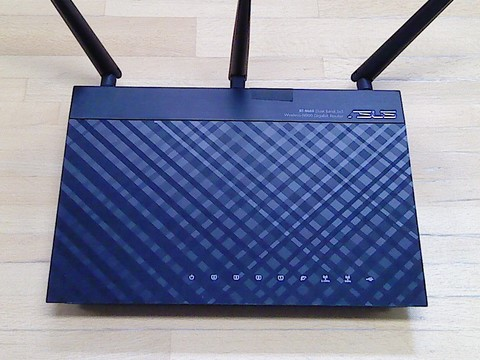
\includegraphics[width=0.35\textwidth]{pics-system/sys-router-front.jpg} &
~ &
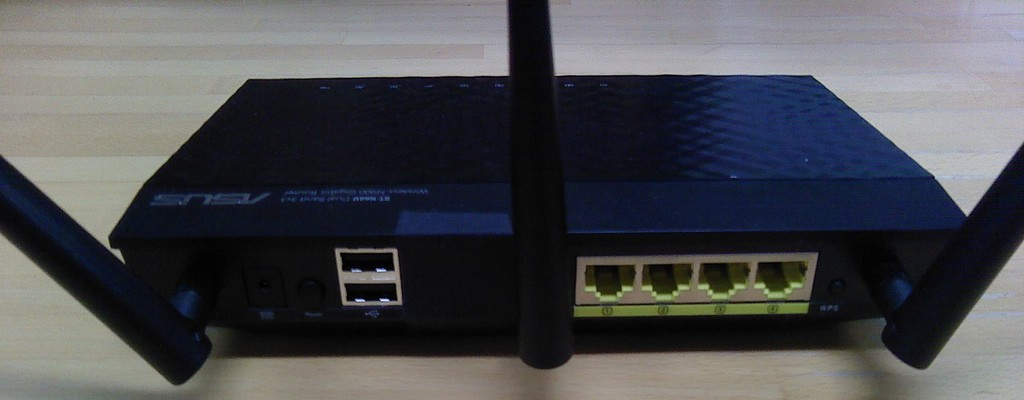
\includegraphics[width=0.45\textwidth]{pics-system/sys-router-back.jpg} \\
\end{tabular}
\end{center}

Changing the administrator login/password (top section):
\begin{center}
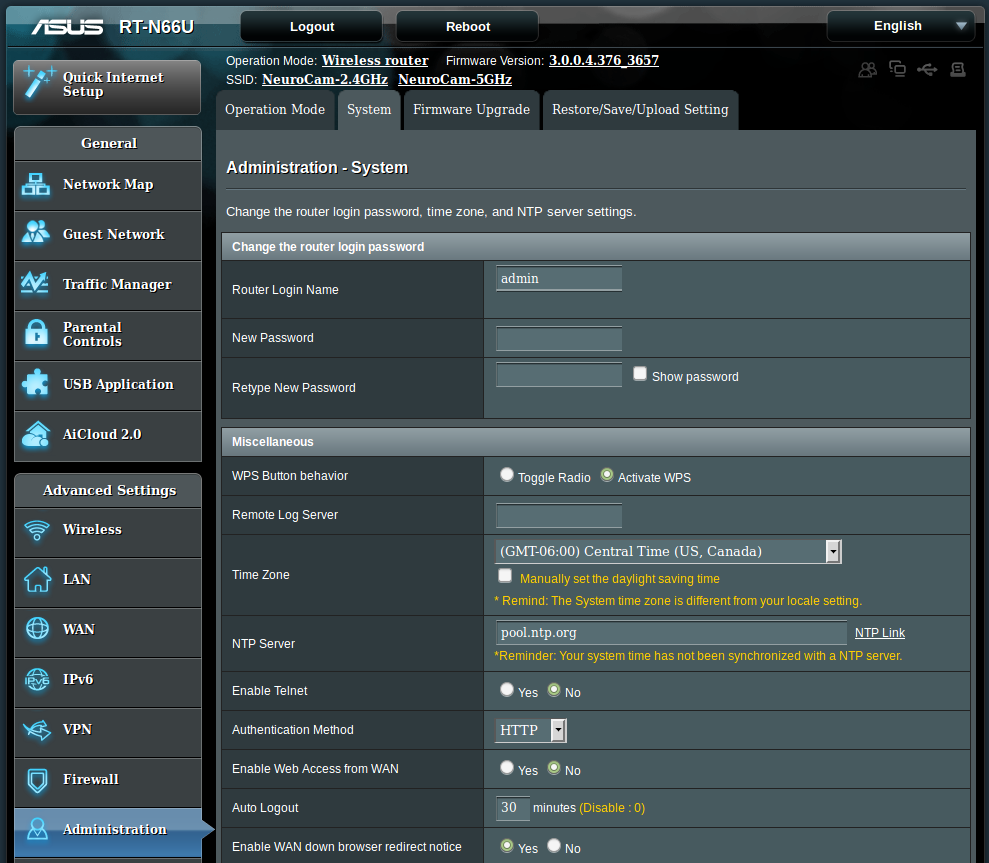
\includegraphics[width=0.7\textwidth]
{pics-router/asus-n66u-admin-pw.png}
\end{center}

% Force a page break.
\clearpage
Setting the wireless network name (``SSID'') and password (``pre-shared 
key''):
\begin{center}
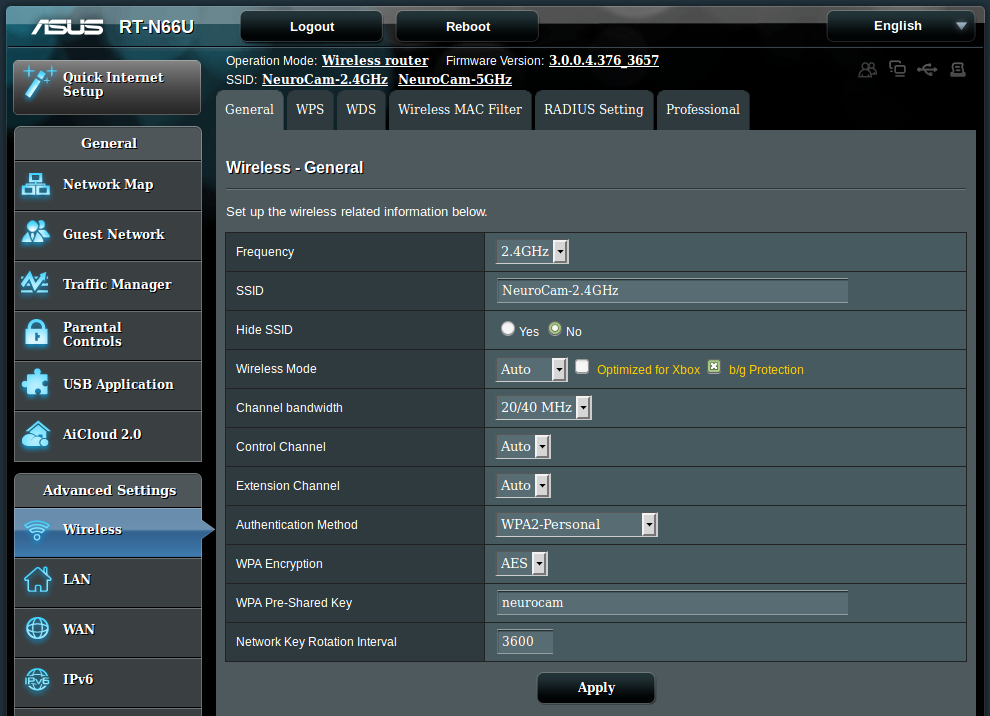
\includegraphics[width=0.7\textwidth]
{pics-router/asus-n66u-ssid.png}
\end{center}

Changing the MAC filter to whitelist mode (``accept the specified 
addresses''), and adding addresses:
\begin{center}
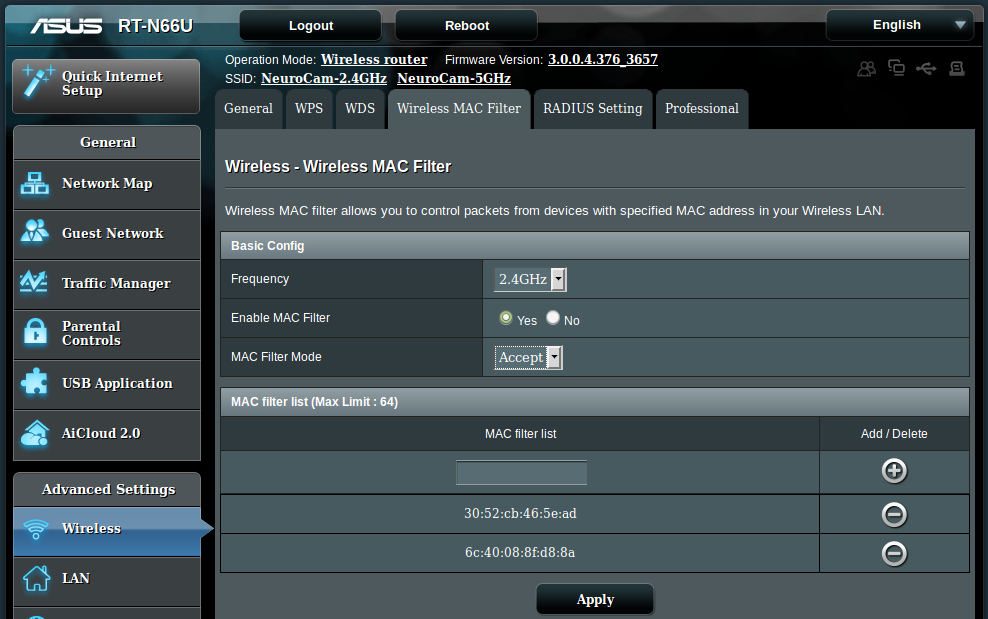
\includegraphics[width=0.7\textwidth]
{pics-router/asus-n66u-macfilter.png}
\end{center}

% Force a page break.
\clearpage
Assigning static IP addresses to specific machines:
\begin{center}
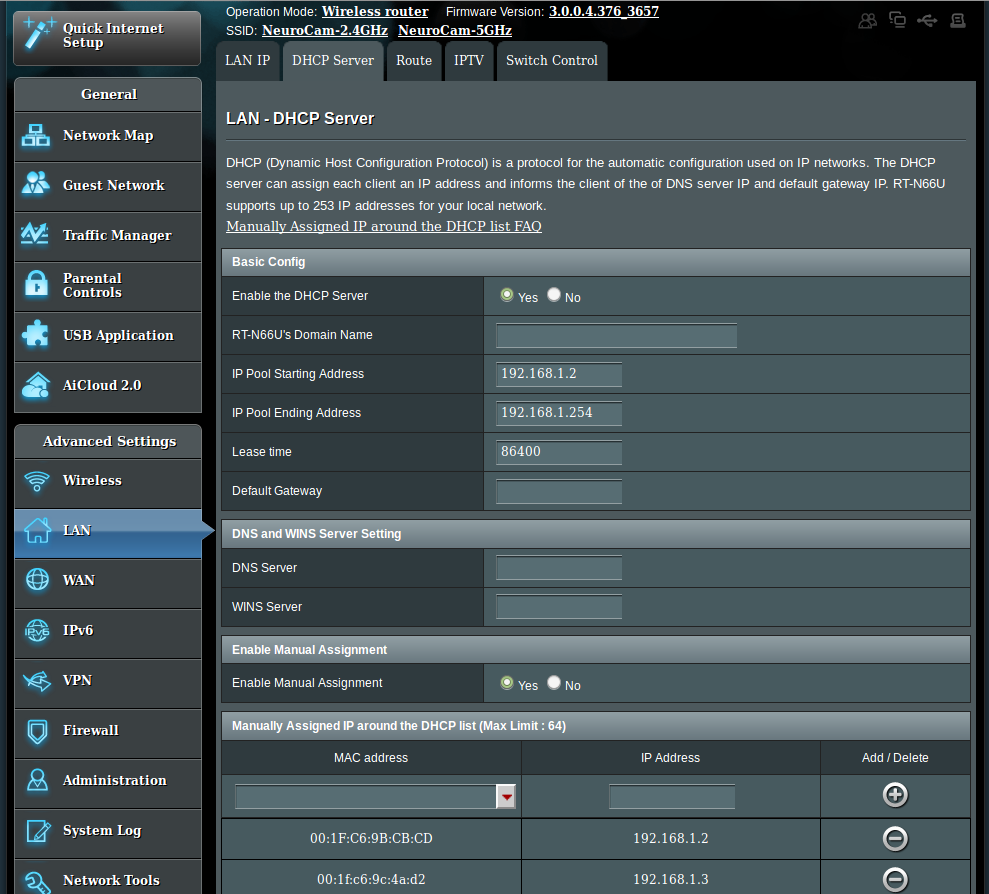
\includegraphics[width=0.7\textwidth]
{pics-router/asus-n66u-static.png}
\end{center}

%
%
\clearpage
\section{Installing OpenWrt}

\fixme{This hasn't been implemented, so no documentation for it.}

{\itshape The idea is to provide scripts that automatically configure and
compile the ``\verb+OpenWrt+'' open--source firmware. This lets us lock down
any features we don't want active, force an appropriate filtering mode, and
disable the web interface (which is one of the main security holes).

Implementing this is deferred, as it will be time--consuming.}

%
% This is the end of the file.
